% !TEX TS-program = pdflatex
% !TEX encoding = UTF-8 Unicode

\documentclass[a4paper, titlepage=false, parskip=full-, 10pt]{scrartcl}

\usepackage[utf8]{inputenc}
\usepackage[T1]{fontenc}
\usepackage[english, ngerman]{babel}
\usepackage{babelbib}
\usepackage{hyperref}
\usepackage{listings}
\usepackage{framed}
\usepackage{color}
\usepackage{graphicx}
\usepackage[normalem]{ulem}
\usepackage{cancel}
\usepackage{amsmath}
\usepackage{amssymb}
\usepackage{amsthm}
\usepackage{algorithm}
\usepackage{algorithmic}
\usepackage{geometry}
\usepackage{subfigure}
\geometry{a4paper, top=20mm, left=35mm, right=25mm, bottom=40mm}

\newcounter{tasknbr}
\setcounter{tasknbr}{1}
\newenvironment{task}[1]{{\bf Aufgabe \arabic {tasknbr}\stepcounter{tasknbr}} (#1):\begin{enumerate}}{\end{enumerate}}
\newcommand{\subtask}[1]{\item[#1)]}

% Listings -----------------------------------------------------------------------------
\definecolor{red}{rgb}{.8,.1,.2}
\definecolor{blue}{rgb}{.2,.3,.7}
\definecolor{lightyellow}{rgb}{1.,1.,.97}
\definecolor{gray}{rgb}{.7,.7,.7}
\definecolor{darkgreen}{rgb}{0,.5,.1}
\definecolor{darkyellow}{rgb}{1.,.7,.3}
\lstloadlanguages{C++,[Objective]C,Java}
\lstset{
escapeinside={§§}{§§},
basicstyle=\ttfamily\footnotesize\mdseries,
columns=fullflexible, % typewriter font look better with fullflex
keywordstyle=\bfseries\color{blue},
% identifierstyle=\bfseries,
commentstyle=\color{darkgreen},      
stringstyle=\color{red},
numbers=left,
numberstyle=\ttfamily\scriptsize\color{gray},
% stepnumber=5,
% numberfirstline=true,
breaklines=true,
% prebreak=\\,
showstringspaces=false,
tabsize=4,
captionpos=b,
% framexrightmargin=-.2\textwidth,
float=htb,
frame=tb,
frameshape={RYR}{y}{y}{RYR},
rulecolor=\color{black},
xleftmargin=15pt,
xrightmargin=4pt,
aboveskip=\bigskipamount,
belowskip=\bigskipamount,
backgroundcolor=\color{lightyellow},
extendedchars=true,
belowcaptionskip=15pt}

%% Enter current values here: %%
\newcommand{\lecture}{Algorithmische Geometrie SS15}
\newcommand{\tutor}{}
\newcommand{\assignmentnbr}{2}
\newcommand{\students}{Julius Auer, Alexa Schlegel}
%%-------------------------------------%%

\begin{document}  
{\small \textsl{\lecture \hfill \tutor}}
\hrule
\begin{center}
\textbf{Übungsblatt \assignmentnbr}\\
[\bigskipamount]
{\small \students}
\end{center}
\hrule

\begin{task}{rotating calipers}
\item[]
Das Berechnen des Durchmessers entspricht dem Finden der antipodalen Punkte mit dem größten Abstand (zur Erinnerung: \emph{toPosition()} wandelt lediglich einen \emph{Point} in einen \emph{Vector} um. Nur Letztere haben eine Länge):
\lstset{language=Java}
\begin{lstlisting}
public double diameter() {
        double max = 0.0d;

        for(PodalPoints p : antipodalPoints()) {
            double d = Math.abs(p.point1.toPosition().substract(p.point2.toPosition()).length());

            if(d > max)
                max = d;
        }

        return max;
    }
\end{lstlisting}
Instanzen der Klasse \emph{PodalPoint} speichern hierbei die Ergebnisse einer Iteration der \emph{RotatingCalipers}. Relevant sind an dieser Stelle nur die antipodalen Punkte \emph{point1} und \emph{point2}, darüber hinaus werden allerdings auch noch die gefundenen Tangenten (zur Visualisierung) sowie die Indizes der Punkte und die Brücken-Eigenschaft der CSL (zur Berechnung der Konvexen Hülle aus ko-podalen Punkten (wie heißen die im Deutschen?)) gespeichert.

Interessanter ist der Aufruf der \emph{RotatingCalipers} (zur Erinnerung: alle Punkte des Polygons liegen in einem Array \emph{points}):
\begin{lstlisting}
    public LinkedList<PodalPoints> antipodalPoints() {
        LinkedList<PodalPoints> result = new LinkedList<PodalPoints>();
        int p1 = 0;
        int p2 = 0;

        // the first antipodal points are given by the points with the min/max x
        // coordinate
        for(int i = 1; i < points.length; i++) {
            if(points[i].compareTo(points[p1]) < 0)
                p1 = i;

            if(points[i].compareTo(points[p2]) > 0)
                p2 = i;
        }

        // the left/right caliper is constructed 'upwards'/'downwards'
        Line caliper1 = new Line(points[p1], new Point(points[p1].getX(), points[p1].getY() + 10.0d));
        Line caliper2 = new Line(points[p2], new Point(points[p2].getX(), points[p2].getY() - 10.0d));
        double rotatedAngle = 0.0d;






        // do until the calipers rotated a total of 180 degrees
        while(rotatedAngle < Math.PI) {
            // for both calipers: compute the angle between the caliper at point
            // p_i and the linesegment p_i->p_(i+1)
            double angle1 = caliper1.angleTo(lines[p1]);
            double angle2 = caliper2.angleTo(lines[p2]);
            angle1 = Math.abs(angle1 > 0 ? 2.0d * Math.PI - angle1 : angle1);
            angle2 = Math.abs(angle2 > 0 ? 2.0d * Math.PI - angle2 : angle2);

            // choose the smaller angle and rotate both calipers by that angle
            double minAngle = Math.min(angle1, angle2);
            caliper1 = new Line(points[p1], caliper1.rotate(points[p1], minAngle).u);
            caliper2 = new Line(points[p2], caliper2.rotate(points[p2], minAngle).u);
            rotatedAngle += minAngle;

            // move the point that lies on the choosen caliper
            if(angle1 < angle2)
                p1 = (p1 + 1) % points.length;
            else
                p2 = (p2 + 1) % points.length;

            result.add(new PodalPoints(p1, p2, points[p1], points[p2], caliper1, caliper2));
        }

        // just in case we rotated slightly more then 180 degrees, check if the
        // first point is a duplicate of the last one
        if(result.getLast().point1 == result.getFirst().point2 && result.getLast().point2 == result.getFirst().point1)
            result.removeFirst();

        return result;
    }
\end{lstlisting}
Neu Implementiert wurden hierfür die Methoden \emph{angleTo()} für \emph{Line}s und \emph{rotate(point, angle)} ebenfalls für \emph{Line}s:
\begin{lstlisting}
    /**
     * Compute the angle between this and another line. Result is positive or
     * negative just as like an atan2 were used.
     * 
     * @param line a line with the direction this line would have if rotated
     *            anticlockwise by the resulting angle
     * @return angle in radians
     */
    public double angleTo(Line line) {
        return Math.atan2(line.u.get(1), line.u.get(0)) - Math.atan2(u.get(1), u.get(0));
    }

    /**
     * Rotate this line around a given point
     * 
     * @param point centre of rotation
     * @param angle angle in radians
     * @return the rotated line
     */
    public Line rotate(Point point, double angle) {
        Vector pos = point.toPosition();
        double cosa = Math.cos(angle);
        double sina = Math.sin(angle);
        Mat2x2 mat = new Mat2x2(cosa, -sina, sina, cosa);

        // shift the line so that 'point' lies at the coordinates center, rotate
        // it around the euler-angle, shift it back
        return new Line(p1.add(pos.multiply(-1)).compose(mat).add(pos),
                p2.add(pos.multiply(-1)).compose(mat).add(pos));
    }
\end{lstlisting}
Die implementierten Testfälle sind visualisiert und animiert. Es lohnt sich trotzdem, das Jar über die Kommandozeile zu starten um ein paar zusätzliche Informationen zu bekommen. Es wird auch ein Test für das finden der Konvexen Hülle zweier Polygone animiert - da hier auch Calipers rotieren gehe ich davon aus, das dies nicht allzu sehr stört - einfach wegklicken.
\begin{figure}[htpb]
\begin{center}
\subfigure{
    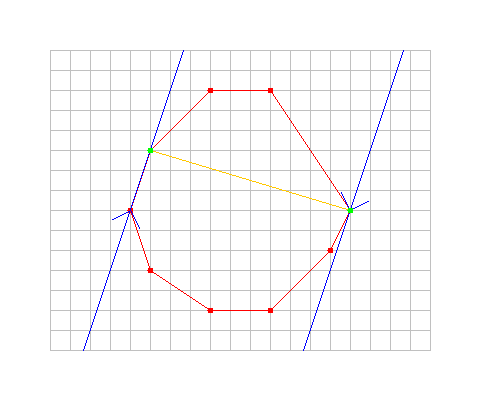
\includegraphics[width=7cm]{capture1}
}
\subfigure{
    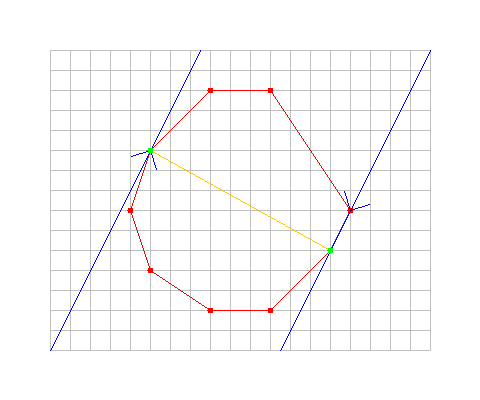
\includegraphics[width=7cm]{capture2}
}
\subfigure{
    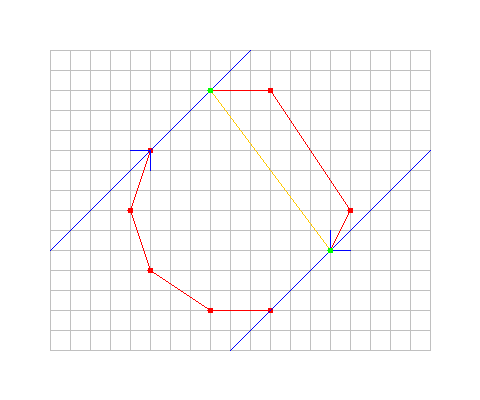
\includegraphics[width=7cm]{capture3}
}
\subfigure{
    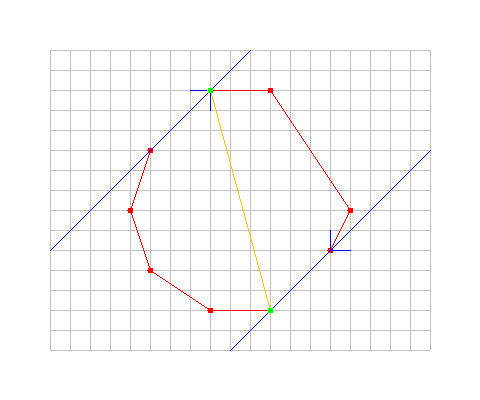
\includegraphics[width=7cm]{capture4}
}
\end{center}
\caption{4 Schleifen-Durchläufe der Rotating Calipers}
\end{figure}
\end{task}
\newpage

\begin{task}{konvexe Hülle}
\subtask{a}
TODO

\subtask{b}
TODO

\end{task}
\end{document}